\setchapterpreamble[u]{\margintoc}
\chapter{Numerical Benchmarks}
\labch{numbench}

In the upcoming sections, we demonstrate the robustness and accuracy of our class of mass-momentum consistent numerical methods when applied to challenging flow configurations involving marked density contrasts, primarily in comparison with the version of our method which does not maintain consistency between the mass and momentum advection. Most of the standard tests that exist in the current literature concerning numerical methods to tackle liquid-gas flows such as the decay of spurious currents in static and moving droplets, viscous damping of capillary waves etc., are carried out in the absence of any density jump (or viscosity jump) across the interface separating the fluids. In this chapter, we shall take a closer look in detail at the behavior of our methods when dealing with difficulties that arise due to the non-linear coupling between interfacial deformation/propagation, capillary and viscous forces, especially in the regime where the material properties across the interface are separated by orders of magnitude, particularly in which the flow features in question are poorly resolved. 

In order to assess the performance of the different methods, we shall use an easier nomenclature to describe the different methods, which are as follows : 

\begin{itemize}
	\item \textbf{STD} : The standard method which does not maintain consistency between mass and momentum transport. 
	\item \textbf{MSHIFT} : The method that ensures consistency between mass and momentum transport, 
		but is not exactly momentum conservative. 
		It is based on the \textit{shifted fractions} strategy, 
		as detailed in the previous chapter. 
	\item \textbf{MSUB} : The method that ensures both consistency between mass and momentum transport, as well as ensuring exactly conservative transport. It uses the \textit{sub-grid} strategy as discussed in the preceding chapter. 
\end{itemize}

%------------------------------------------ STATIC DROP ---------------------------------------------

\section{Static Droplet}
\labsec{static}

A popular numerical benchmark in the existing literature relevant to surface tension dominated flows is the case of a spherical droplet of the denser fluid immersed in a quiescent surrounding medium of the lighter fluid. In the hydrostatic limit of the Navier-Stokes equations, the droplet should stay in equilibrium, with a curvature induced pressure jump across the interface corresponding to Laplace's equilibrium. In practice however, numerically reproducing such a trivial equilibrium condition is not as straighforward, as there exists a slight difference between the initial numerical interface and the exact analytical shape of the sphere, thereby resulting in the generation of the well documented '\textit{spurious}' or '\textit{parasitic}' currents of varying intensity in the velocity field \sidecite{lafaurie1994modelling, harvie2006analysis, popinet1999front}. A lot or progress has been made since in the context of \textit{well-balanced} surface tension formulations, that ensure consistency between the numerical stencils used for the discretization of the pressure gradient and the Heaviside approximation ($n \delta_{s}$) that projects the the surface force distribution onto the control volumes \cite{francois2006balanced,popinet2009accurate}. A significant contribution to the interpretation of these parasitic currents within the well-balanced framework was made by Popinet \cite{popinet2009accurate} which demonstrated that given sufficient time (of the order of viscous dissipation time-scales), a well-balanced method will relax to the '\textit{numerical}' equilibrium shape through the damping of the 'physically consistent' numerical capillary waves, therefore allowing us to recover the exact (to machine precision) Laplace equilibrium condition.

\subsection*{Setup}

% insert figure  

\begin{figure}[h!]
    \centering
    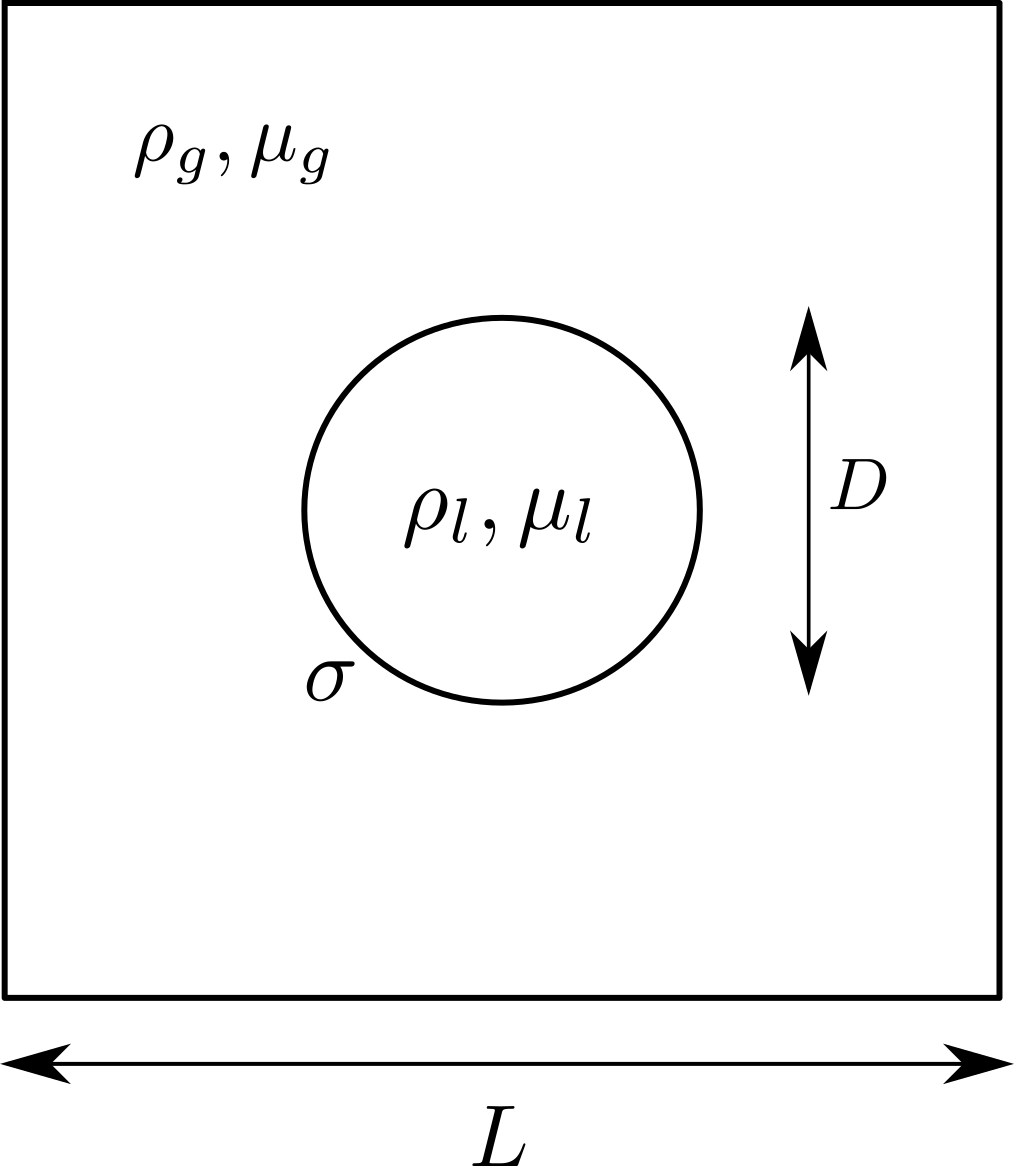
\includegraphics[width = 1.0\textwidth]{plots/static_drop/config.png}
    \caption{Schematic of the static droplet of dense fluid surrounded by a quiescent medium of lighter fluid. A $40 \times 40$ grid is employed to spatially discretize the domain.}
    \label{static_conf}
\end{figure}

% difference in our setup in terms of high-density ratios
The key difference in our implementation of this classic test case from that of Popinet \sidecite{popinet2009accurate} is that we consider the effect of density contrast across the interface separating the fluids. As we have previously discussed, a sharp density jump across the interface may have an amplification effect on the numerical errors incurred as a result of interfacial reconstructions, curvature estimation and various other truncations, thereby rendering the method unstable. We demonstrate that in our framework of mass consistent momentum transport coupled with a well-balanced surface tension discretization, density-ratios as large as $1000:1$ can be simulated without loss of numerical stability, in conjuction with the ability to recover the exact numerical equilibrium through the dissipation of spurious currents within relevant time-scales \sidenote{The viscous time-scale corresponding to the droplet length-scale is the most commonly used in literature.}.

% specification of numerical problem setup, domain, densities and viscosities
We consider a circular droplet of size $D$  placed at the centre of a square domain of side $L$. The densities of the heavier and lighter phases are $\rho_l$ and $\rho_g$ respectively, likewise for the viscosities $\mu_l$ and $\mu_g$, and $\sigma$ being the surface tension coefficient (fig. \ref{static_conf}). The ratio of the droplet size to the box is chosen as $D/L = 0.4$, coupled with a numerical resolution of $D/\Delta x= 16$ (where $\Delta x$ is the grid size). As for boundary conditions, we use symmetry conditions on all sides of the square domain.

% specification of problem parameters and adimensional numbers 
The problem incorporates two natural time-scales, the capillary oscillation scale and the viscous dissipation scale, which are defined below :

\begin{align}
        T_\sigma = \left(\frac{\rho_l D^3}{\sigma}\right)^{1/2} \quad , \quad T_\mu = \frac{\rho_l D^2}{\mu_l}
\label{ts}
\end{align}

The ratio of these time-scales give us -

\begin{align}
        \frac{T_\mu}{T_\sigma} = \sqrt{\rho_l \sigma D}/\mu_l = \sqrt{La}
\end{align}

where $La$ is the Laplace number based upon the heavier fluid. In the present study, we introduce the density-ratio $\rho_l/\rho_g$ as another important parameter. In order to rescale our 'parasitic' velocity field, we define a velocity scale based on capillary oscillations as -

\begin{align}
        U_\sigma = \sqrt{\sigma/\rho_l D}
\end{align}

Additionally, the time-step in our numerical simulation must be smaller than the oscillation period corresponding to the grid wavenumber (fastest capillary wave with a time period $\sim \left( \rho_l \Delta x^3 / \sigma  \right)^{1/2} $ ) as a stability criterion \sidenote{Similar criteria are defined on the basis of the viscous and advection operators as well, with the smallest amongst the three selecting the numerical time-step}, as our surface tension model is explicit in time. For the scope of the present study, we shall not consider any viscosity contrast between the two fluids while varying the density-ratio, therefore $\mu_l/\mu_g = 1$ for all the cases under study.


\subsection*{Decay of Spurious Currents}

In figures \ref{decay_nonmc} to \ref{decay_sagar}, we illustrate the decay of the root-mean-square of the spurious currents as a function of time, in the case of four different density-ratios, with three different Laplace numbers for each ratio. The first figure (\ref{decay_nonmc}) refers to simulations carried out without consistency between the momentum-mass transport (\textbf{STD}), the second (\ref{decay_daniel}) corresponds to that of the consistent but not conservative method (\textbf{MSHIFT}), and final one (\ref{decay_sagar}) refers to that of the consistent and conservative method (\textbf{MSUB}). The time is rescaled by the viscous dissipation scale, and the spurious currents by the capillary velocity scale. We have two main observations, the rapid decay of the rescaled spurious currents for all combinations of density-ratios and Laplace numbers within approximately $0.2 T_{\mu}$, and the slower re-growth of the currents in question for combinations of non-unity density-ratios and large Laplace numbers, in all simulations except those carried out with \textbf{MSUB}. With method \textbf{MSUB}, the decayed currents keep hovering around levels of machine precision for remainder of time. Although there is a re-growth of the currents using the consistent method (\textbf{MSHIFT}) after $0.2 T_{\mu}$, the behavior is not quite alarming as the rate of this re-growth is quite low. Therefore, out of all the methods tested, the consistent and conservative method (\textbf{MSUB}) does seem to demonstrate the desired performance, especially when it comes to combinations of large density contrasts coupled with large Laplace numbers.   


\begin{figure}[h!]
    \centering
    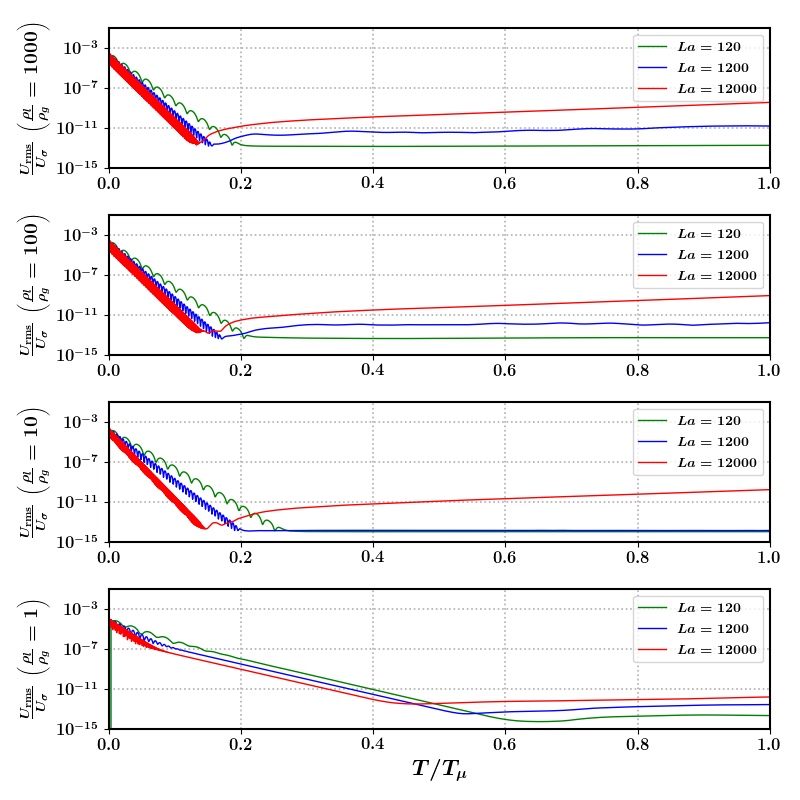
\includegraphics[]{plots/static_drop/decay_nonmc.png}
	\caption{\textbf{STD} Decay of normalized spurious currents as a function of viscous dissipation time-scales for different density-ratios and Laplace numbers. The currents seem to initially decay quickly for all higher density-ratios, and relax to the numerical equilibrium curvature even within $0.2 \cdot T_\mu$. For combinations of large $\rho_l / \rho_g$ and large $La$, the spurious currents seem to grow back to an order of magnitude ($10^{-8}$) which is quite far from that of machine precision ($10^{-14}$).}   
    \label{decay_nonmc}
\end{figure}

\begin{figure}[h!]
    \centering
    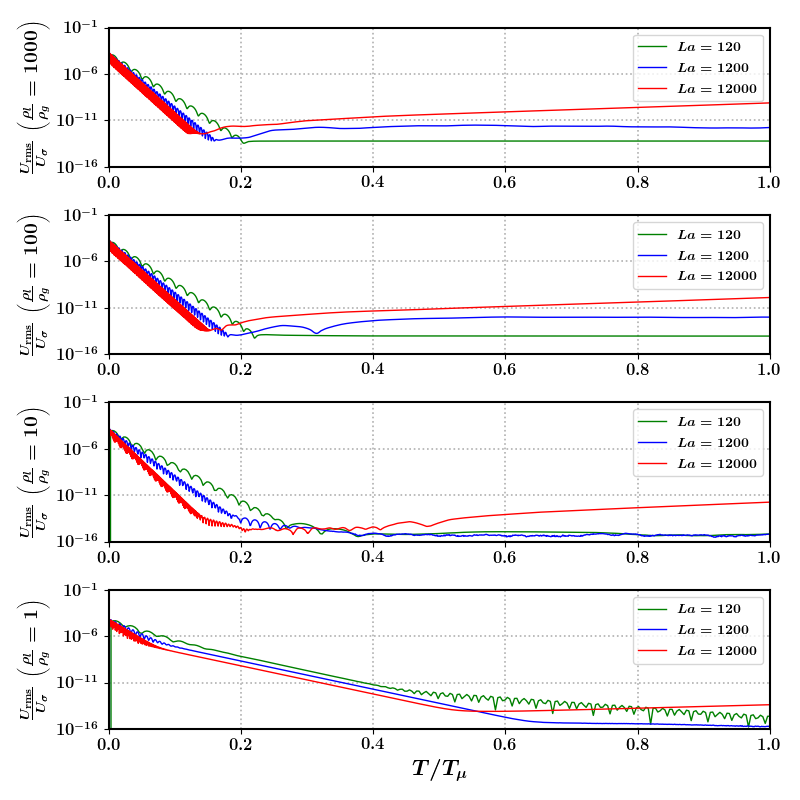
\includegraphics[]{plots/static_drop/decay_daniel.png}
	\caption{\textbf{MSHIFT} Decay of normalized spurious currents as a function of viscous dissipation time-scales for different density-ratios and Laplace numbers. The currents seem to initially decay quickly for all higher density-ratios, and relax to the numerical equilibrium curvature even within $0.2 \cdot T_\mu$. For combinations of large $\rho_l / \rho_g$ and large $La$, the spurious currents seem to grow back to an order of magnitude ($10^{-8}$) which is quite far from that of machine precision ($10^{-14}$). No considerable improvement is observed with respect to \textbf{STD}. }   
    \label{decay_daniel}
\end{figure}

\begin{figure}[h!]
    \centering
    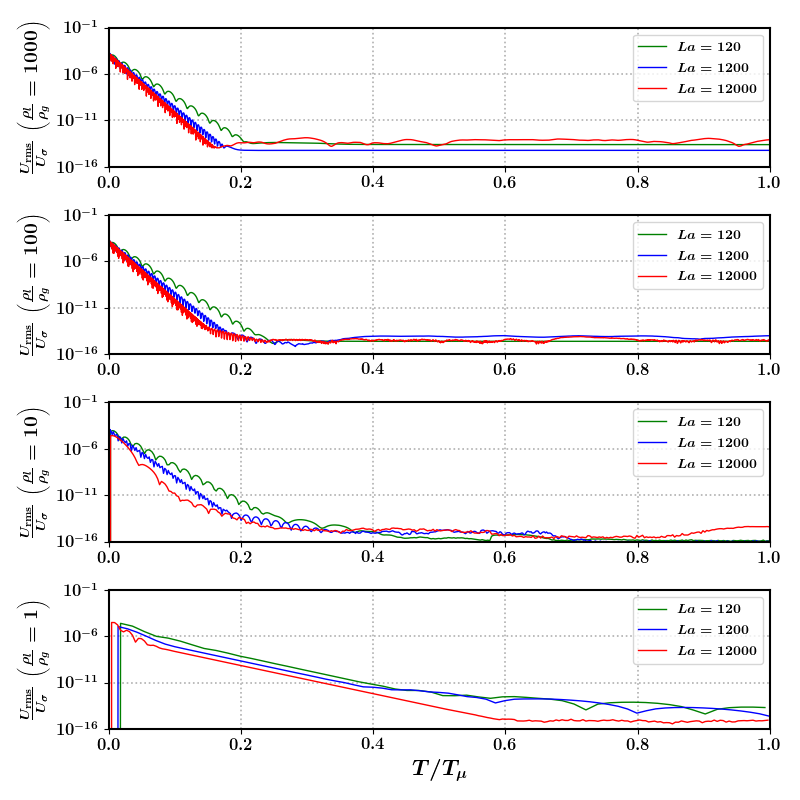
\includegraphics[]{plots/static_drop/decay_sagar.png}
	\caption{\textbf{MSUB} Decay of normalized spurious currents as a function of viscous dissipation time-scales for different density-ratios and Laplace numbers. The currents seem to decay very quickly in the case of higher density-ratios, and relax to the numerical equilibrium curvature even within $0.2 \cdot T_\mu$. For all combinations of $\rho_l / \rho_g$ and $La$ numbers, the decayed spurious currents are not observed to grow back as in the cases of \textbf{STD} and \textbf{MSHIFT}, and hover around values close to machine precision ($10^{-14}$).}   
    \label{decay_sagar}
\end{figure}



\subsection*{Spatial Convergence}

Once the solution relaxes to a numerical equilibrium curvature (spurious currents are approximately at the order of machine precision), there still exists a difference between the numerical curvature and the exact analytical curvature corresponding to the spherical (circular) shape. We use the definitions of the shape errors as introduced in the seminal work of Popinet \cite{popinet2009accurate} to assess the convergence of our class of methods to the exact (analytical) curvature as we increase spatial resolution. The norms are defined as follows :      

\begin{align}
	L_2 = \sqrt{\frac{\sum_i \left(C_i - C_i^\text{exact} \right)^2}{\sum_i}} \quad , \quad L_\infty = \text{max}_i \left( | C_i - C_i^\text{exact} | \right)
  \label{shape_err_norms}
\end{align}

where $C_i$ is the volume fraction of a cell after the solution has relaxed to the numerical equilibrium curvature, and $C_i^\text{exact}$ is the volume fraction corresponding to the exact circular shape which was initialized at the start of the simulation.  

Fig. \ref{static_drop_conv} demonstrates the behavior of the shape errors defined in eqn. \ref{shape_err_norms} for the case of the most stringent parameter combination ( $\rho_l / \rho_g = 1000 $ , $La = 12000$ ) as a function of the droplet resolution. As one can clearly observe, all the methods tested display a roughly second-order convergence in space for both the error norms. In terms of the $L_2$ norm, the consistent and conservative method (\textbf{MSUB}) does indeed achieve smaller errors as compared to both \textbf{STD} and \textbf{MSHIFT} for all spatial resolutions. As a minor remark, there is not much to discern in terms of shape error when it comes to comparing the performances of the consistent (\textbf{MSHIFT}) method with the non-consistent one (\textbf{STD}). 

\begin{figure}[h!]
    \centering
    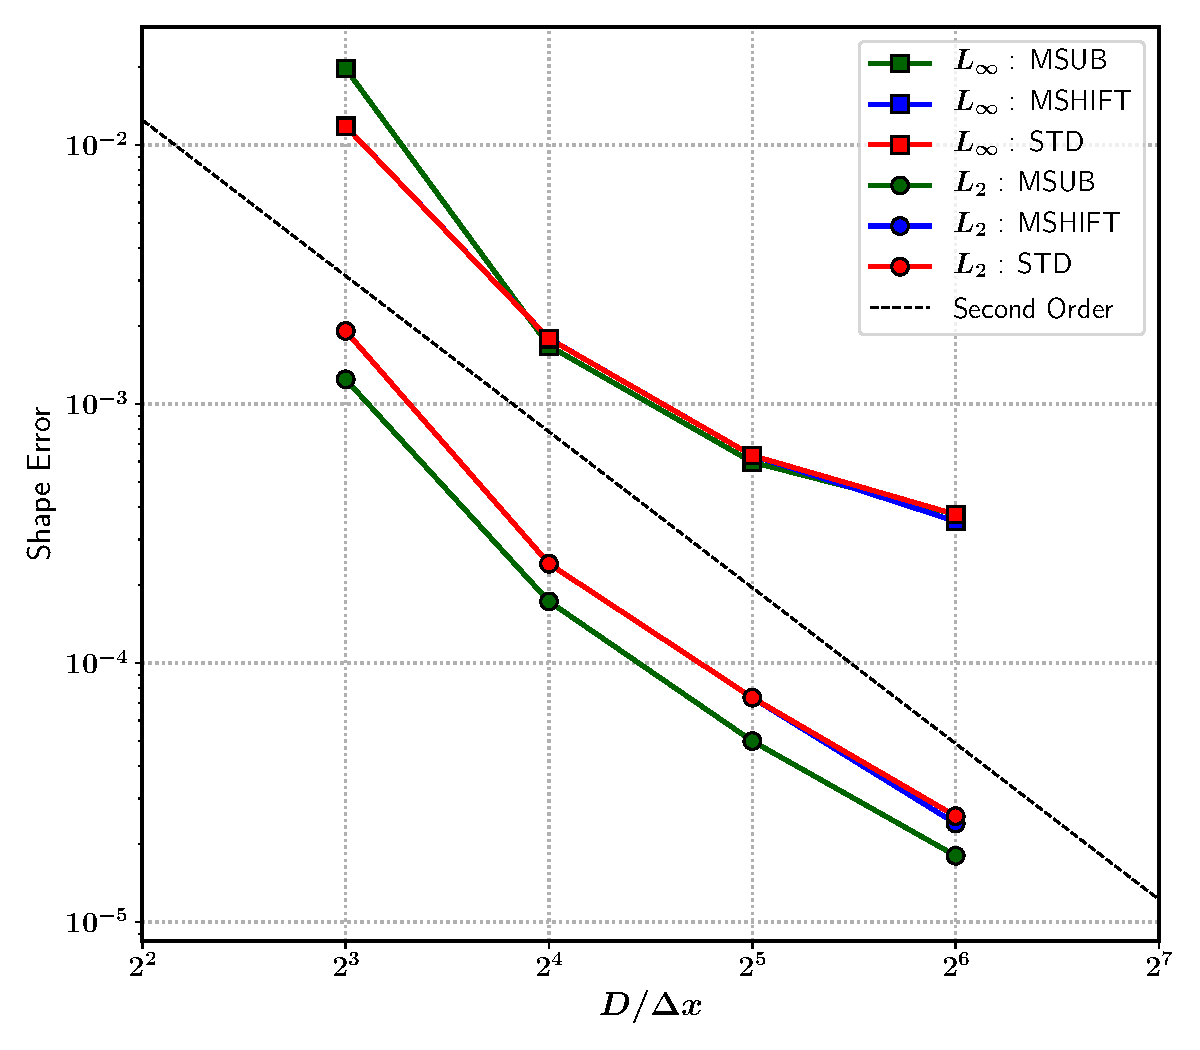
\includegraphics[width = 1.0\textwidth]{plots/static_drop/convergence.pdf}
	\caption{Second-order spatial convergence for the spurious current error norms corresponding to the most stringent parameter combination ($\rho_l/\rho_g = 1000$ , $La = 12000$) . Both of the norms ($L_\infty$ and $L_2$) seem to demonstrate a roughly second order rate of spatial convergence with each of the methods tested. However, \textbf{MSUB} has a marginally lower $L_2$ error compared to both \textbf{STD} and \textbf{MSHIFT} for all resolutions tested. There is negligible difference observed in the shape errors between \textbf{STD} and \textbf{MSHIFT} in both of the norm definitions.}   
    \label{static_drop_conv}
\end{figure}


%------------------------------------------ MOVING DROP ---------------------------------------------

\section{Moving Droplet}

An incisive numerical setup that enables us to evaluate the accuracy of the coupling between interfacial propagation and surface tension discretization was first proposed by Popinet \cite{popinet2009accurate}, and subsequently employed in the comparative study of Abadie et al. \sidecite{abadie2015combined}. The manner in which this test differs from that of the static droplet is the addition of a uniform background velocity field, therefore serving as a better representation of droplets in complex surface tension dominated flows where they might be advected by the mean flow. In terms of the Laplace equilibrium, the hydrostatic solution is still valid in the frame of reference of the moving droplet. The point at which the solution in the moving reference frame diverges from that of the static droplet (\ref{sec:static}) is through the continuous injection of noise at the scale of the grid size. This 'numerical' noise emanates from the perturbations to the curvature estimates, which are in turn induced by the interfacial reconstructions carried out to propagate the interface (temporal integration) . These fluctuating errors act as source terms for the momentum, thereby transforming the problem into that of viscous dissipation in the presence of continuous forcing (in the reference frame of the moving drop).

\subsection*{Setup}

\begin{figure}[h!]
    \centering
    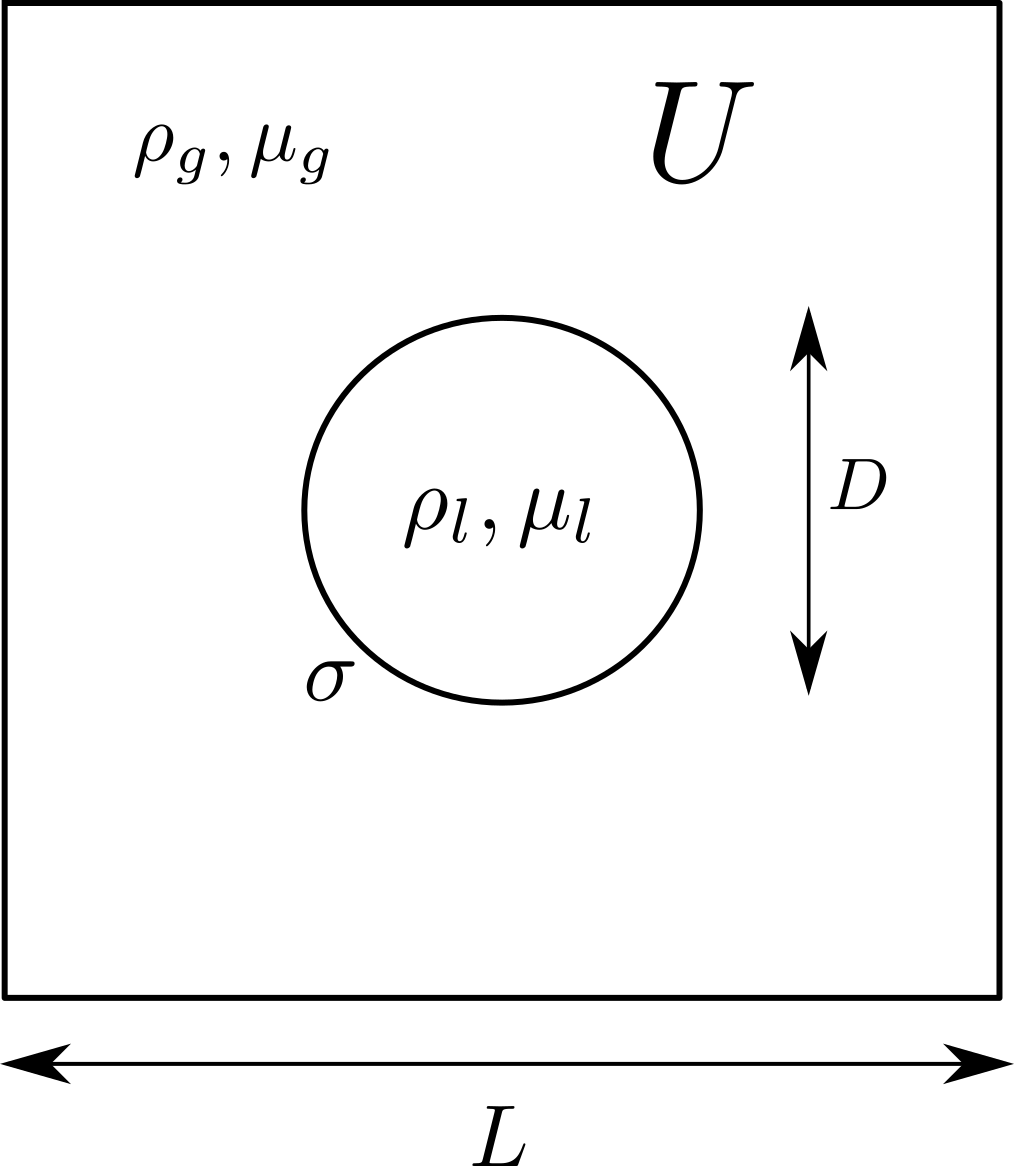
\includegraphics[width = 1.0\textwidth]{plots/droplet_advect/config.png}
    \caption{Schematic of the droplet of dense fluid advected in a surrounding medium of lighter fluid. A $50 \times 50$ grid is employed to spatially discretize the domain, which is spatially periodic in the direction of droplet advection.}
    \label{moving_conf}
\end{figure}

In the present study, we evaluate our class of methods using the advection of a droplet in a spatially periodic domain using an identical setup as \cite{popinet2009accurate}, but with the important difference of including sharp density jumps across the interface as well as using lower spatial resolutions. As previously discussed (\ref{sec:static}), large density contrasts tend to amplify the fluctuations induced by the myriad numerical approximations (interface reconstruction, curvature estimation etc) involved in the algorithm.

We consider a circular droplet of diameter $D$ placed at the centre of a square domain of side $L$. The densities of the heavier and lighter phases are $\rho_l$ and $\rho_g$ respectively, likewise for the viscosities $\mu_l$ and $\mu_g$, and $\sigma$ being the surface tension coefficient (fig. \ref{moving_conf}). A uniform velocity field $\boldsymbol{U}$ is initialized on the entire domain (only a horizontal component). The ratio of the droplet size to the box is $D/L = 0.4$, with $D/\Delta x= 20$ ($\Delta x$ being the grid size. \sidenote{In Popinet \cite{popinet2009accurate}, a resolution of $D / \Delta x = 25.6$ corresponding to a grid of $64 \times 64$ is used } ). As for boundary conditions, we use symmetry conditions on the top and bottom sides, and periodic boundary conditions on the horizontal direction (along which advection by $U$ takes place). We characterize by problem by introducing the following adimensional parameters (based on the heavier fluid) :

\begin{align}
        La = \frac{\rho_l \sigma D}{\mu_l^2} \quad , \quad We = \frac{\rho_l U^2 D}{\sigma}
\end{align}

In addition to the capillary and viscous time-scales for the static case (eqns. \ref{ts}), we have an additional scale defined as :

\begin{align}
	T_{u} = D/U
\end{align}

which is the time-scale of advection. In our subsequent analysis, we shall use $T_u$ and $U$ as the time and velocity scales, repectively.

\subsection*{Evolution of Spurious Currents}

\begin{figure}[h!]
    \centering
    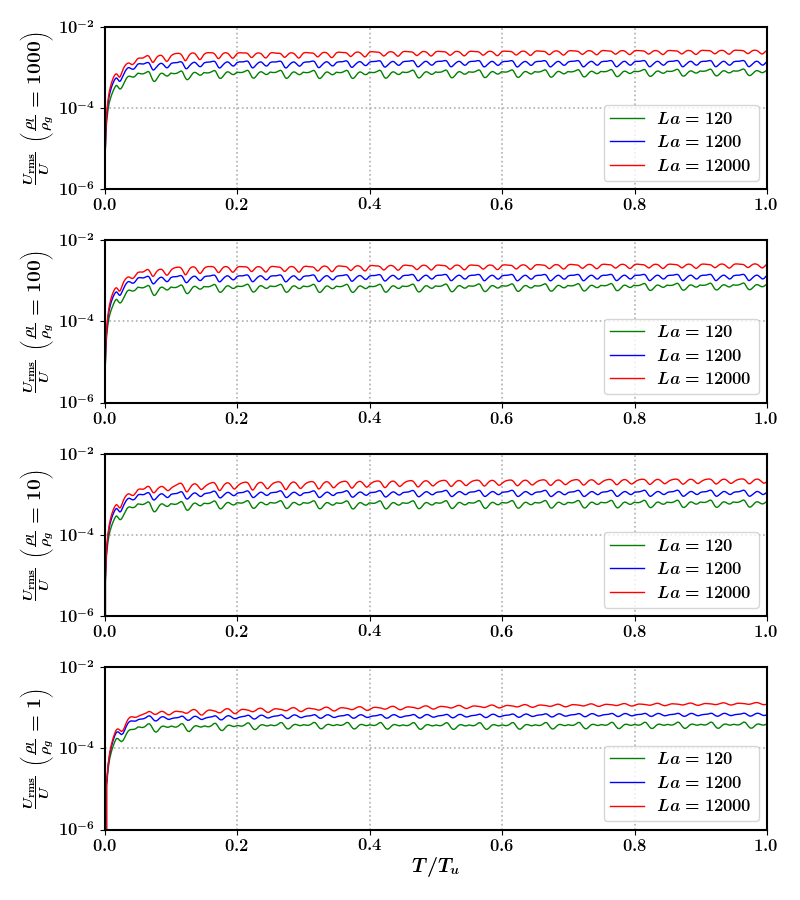
\includegraphics[]{plots/droplet_advect/evo_nonmc.png}
	\caption{\textbf{STD} Time evolution of normalized spurious currents as a function of advection time-scales ($T_u$) for different combinations of density-ratio and Laplace numbers. The currents seem to hover around $10^{-3}$, with a larger Laplace number corresponding to a higher error for all density-ratios. $We = 0.4$ for all the cases presented.}   
    \label{evo_nonmc}
\end{figure}

\begin{figure}[h!]
    \centering
    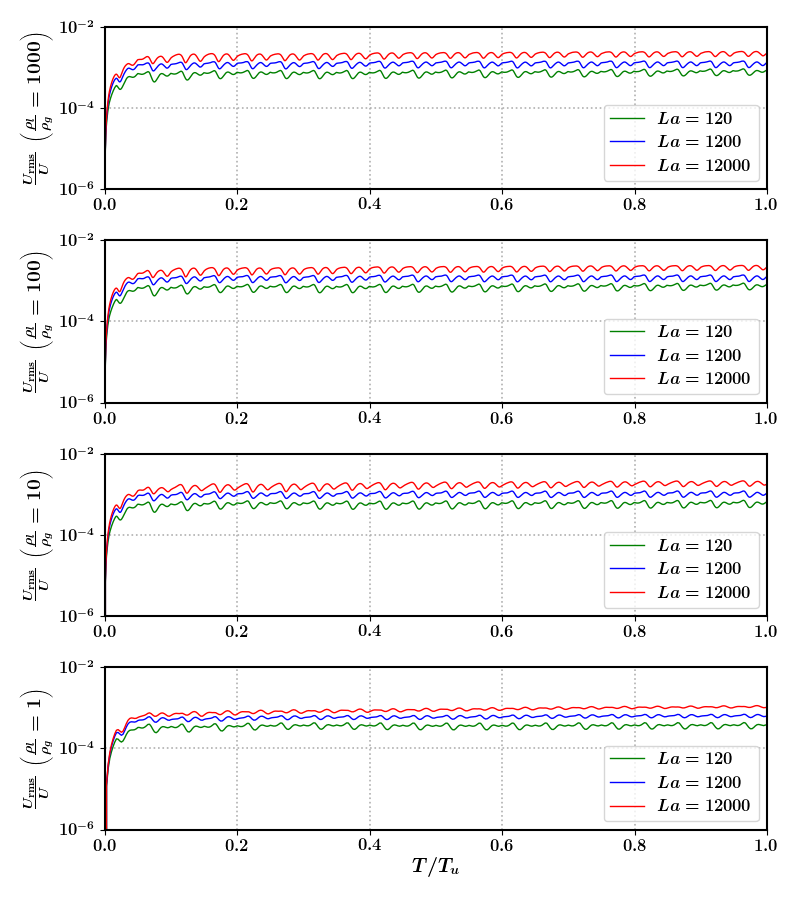
\includegraphics[]{plots/droplet_advect/evo_daniel.png}
	\caption{\textbf{MSHIFT} Time evolution of normalized spurious currents as a function of advection time-scales ($T_u$) for different combinations of density-ratio and Laplace numbers. There seems to be no appreciable difference from the evolution seen in the case of \textbf{STD} (fig. \ref{evo_nonmc}). The currents seem to hover around $10^{-3}$, with a larger Laplace number corresponding to a higher error for all density-ratios. $We = 0.4$ for all the cases presented.}   
    \label{evo_daniel}
\end{figure}

\begin{figure}[h!]
    \centering
    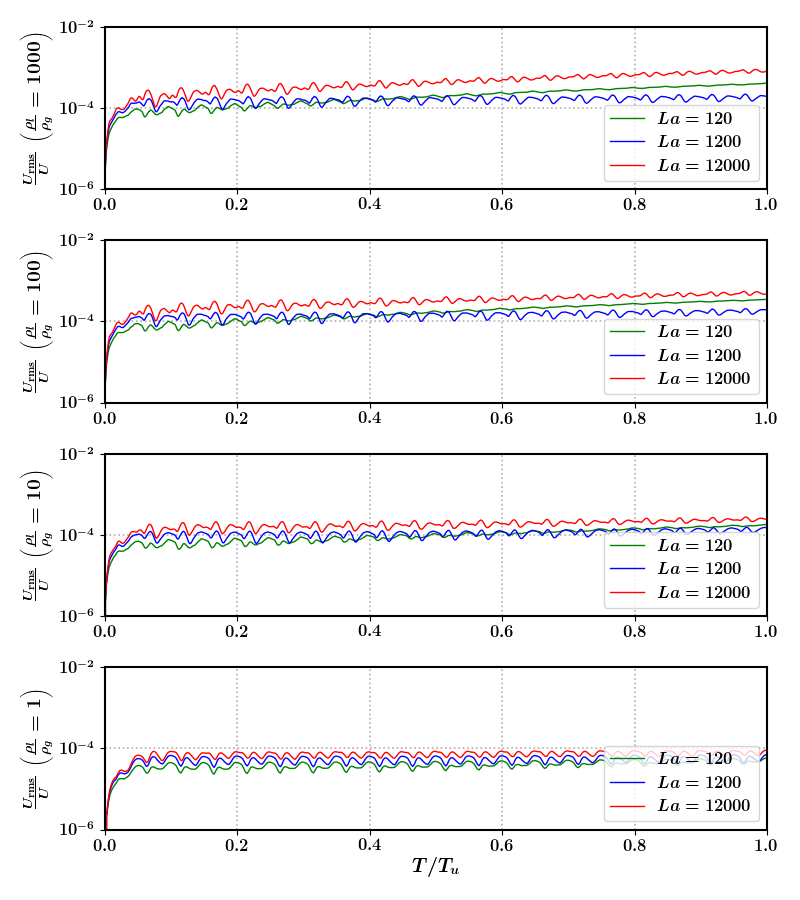
\includegraphics[]{plots/droplet_advect/evo_sagar.png}
	\caption{\textbf{MSUB} Time evolution of normalized spurious currents as a function of advection time-scales ($T_u$) for different combinations of density-ratio and Laplace numbers. In terms of the errors observed in \textbf{STD} and \textbf{MSHIFT}, we observe a decrease of roughly one order of magnitude. Although an upward trend is observed for large Laplace numbers, the growth rate is quite low. The currents seem to hover slightly above $10^{-4}$, with larger Laplace numbers corresponding to larger errors for all density-ratios. $We = 0.4$ for all the cases presented.}   
    \label{evo_sagar}
\end{figure}

Figures \ref{evo_nonmc} to \ref{evo_sagar} depict the evolution of the root-mean-square (RMS) error of the velocity field in the moving frame of reference, as a function of different Laplace numbers, spanning over density ratios separated by orders of magnitude. The first figure (\ref{evo_nonmc}) refers to simulations carried out without consistency between the momentum-mass transport (\textbf{STD}), the second (\ref{evo_daniel}) corresponds to that of the consistent but not conservative method (\textbf{MSHIFT}), and final one (\ref{evo_sagar}) refers to that of the consistent and conservative method (\textbf{MSUB}). We again have a couple of important observations, the first being that spurious currents do not decay to machine precision as in the static droplet case for all of the combinations and methods tested, instead they oscillate around a mean value of the order of $(0.1-0.01)\% $ of the constant field $U$. The second observation is regarding the significantly smaller error (almost by one order of magnitude) in the case of the consistent and conservative method (\textbf{MSUB}) when compared to that of \textbf{STD} and \textbf{MSHIFT}. As a minor remark, in case of large Laplace numbers, the \textbf{MSUB} method displays a slight upward trend in the error evolution, which is not the case in either \textbf{STD} or \textbf{MSHIFT}. This is not too worrisome as the growth is over a time-scale much larger than $T_u$, with the oscillations corresponding to a time-scale of the order $U/\Delta x$. All of the plots in figures \ref{evo_nonmc} to \ref{evo_sagar} correspond to $We = 0.4$, alongside an additional simplification of equal viscosities across the interface i.e $\mu_l/\mu_g = 1$ .

As evindenced by the persistence of these spurious currents due to the addition of grid-level noise emanating from interfacial reconstructions, further advancements should be made with respect to the combined performace of the interfacial transport, curvature computation and the surface tension model. Nonetheless, all the methods tested do seem to be quite numerically stable when dealing with the high density-ratios, and are not subject to rapid uncontrollable amplifications of the interfacial perturbations even for high Laplace numbers.

\subsection*{Spatial Convergence}

In order to evaluate the performance of our class of methods at different resolutions, we define the errors as the maximum values of the norms $L_\infty$ and $L_2$ of the rescaled field $U_{rms}/U$ over time ($5$ times $T_u$). In fig. \ref{moving_drop_conv}, we show the scaling of the error as a function of spatial resolution for the most stringent case of $\rho_l/\rho_g = 1000 $ , $La = 12000$, for each of our different methods. As similarly observed in section \ref{sec:static}, in terms of both $L_\infty$ and $L_2$ norms, there is no appreciable difference in the behaviors of \textbf{STD} and \textbf{MSHIFT}. For \textbf{MSUB}, we do observe significantly lower maximum errors compared to other two methods, but at a cost of slightly less than first-order convergence. The overall convergence behavior of the class of methods we have tested seems to be consistent with earlier studies of Popinet \cite{popinet2009accurate} and others \sidenote{In existing literature, convergence rates have only been studied in case of equal density fluids across the interface} .  

\begin{figure}[h!]
    \centering
    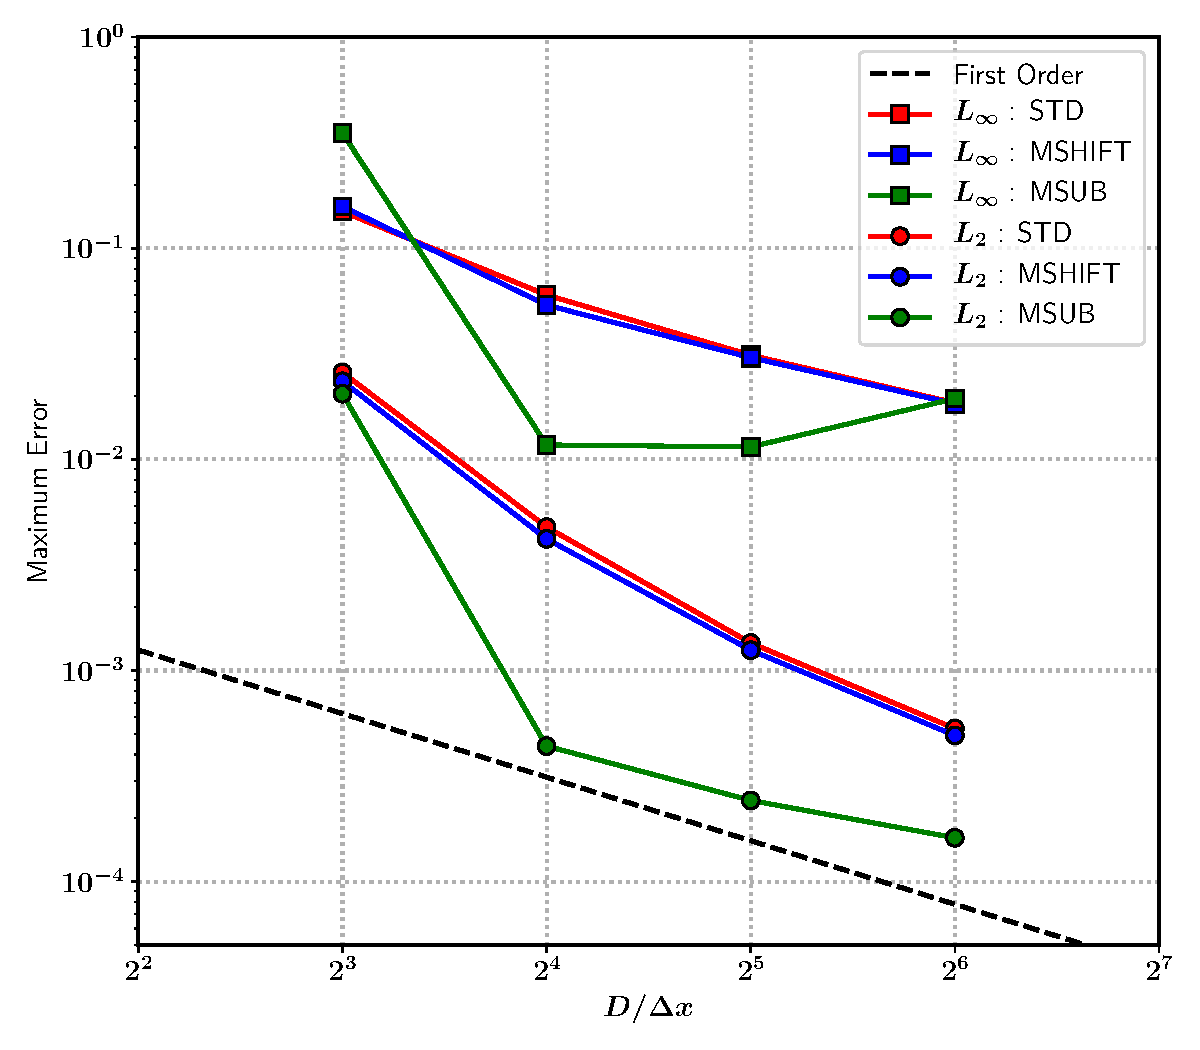
\includegraphics[width = 1.0\textwidth]{plots/droplet_advect/convergence.pdf}
	\caption{First-order (approximately) spatial convergence of the maximum of the spurious current error norms in the frame of reference of the moving droplet, for the most stringent parameter combination ($\rho_l/\rho_g = 1000 $ , $La = 12000$, $We = 0.4$). Methods \textbf{STD} and \textbf{MSHIFT} display similar convergence properties, whereas \textbf{MSUB} leads to significantly lower errors even though it doesn't quite follow the first-order convergence rate. }   
    \label{moving_drop_conv}
\end{figure}

\subsection*{Error Dependence : Laplace \& Weber numbers}

As the final point of inquiry into the performance of our class of methods, figures \ref{web} and \ref{lap} demonstrate the influence of the Laplace and Weber numbers on the behavior of the maximum error norm, carried out for the largest density-ratio ($\rho_l/\rho_g = 1000$). We present results obtained using the consistent and conservative method (\textbf{MSUB}), for a resolution corresponding to $D / \Delta x = 25.6$. As we can observe, the error (both $L_\infty$ and $L_2$) scales as $We^{-1/3}$ over 4 orders of magnitude, which is different from the $We^{-1/2}$ scaling observed by Popinet \cite{popinet2009accurate} \sidenote{ Although Popinet \cite{popinet2009accurate} had equal densities ($\rho_l/\rho_g = 1$) }. In terms of Laplace numbers, the errors scale as $La^{1/6}$ over two orders of magnitude, which is the same as that observed in \cite{popinet2009accurate} (for equal densities).

\begin{figure}
    \centering
    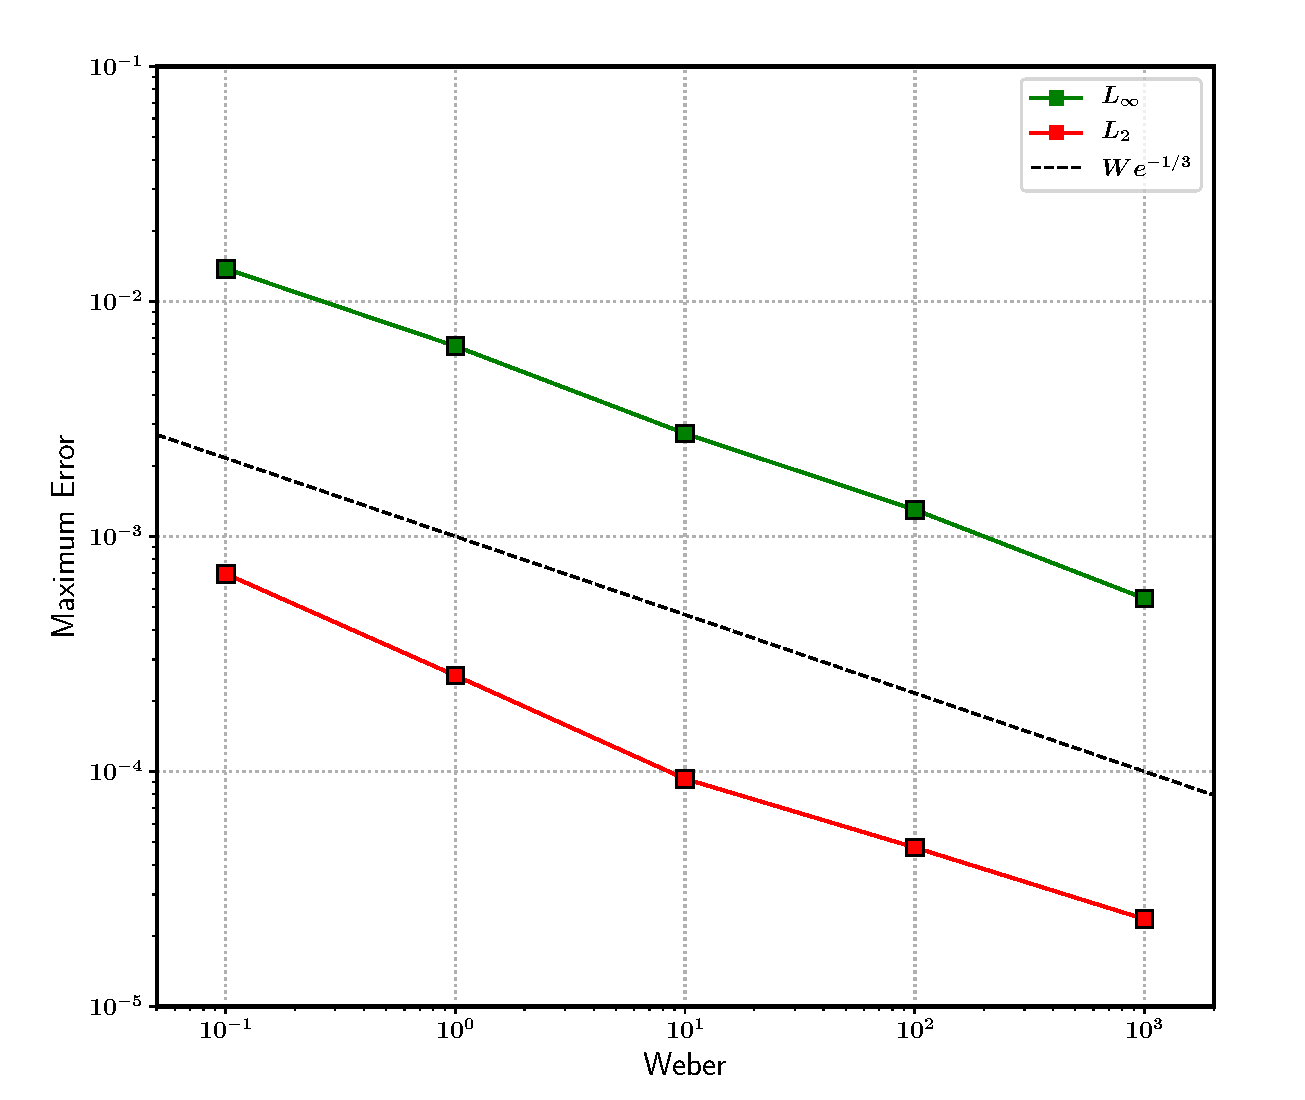
\includegraphics[width = 1.0\textwidth]{plots/droplet_advect/webers.pdf}
\caption{ Scaling of the maximum error norm as a function of Weber ($La = 12000$, $\rho_l / \rho_g = 1000$). }
    \label{web}
\end{figure}

\begin{figure}
    \centering
    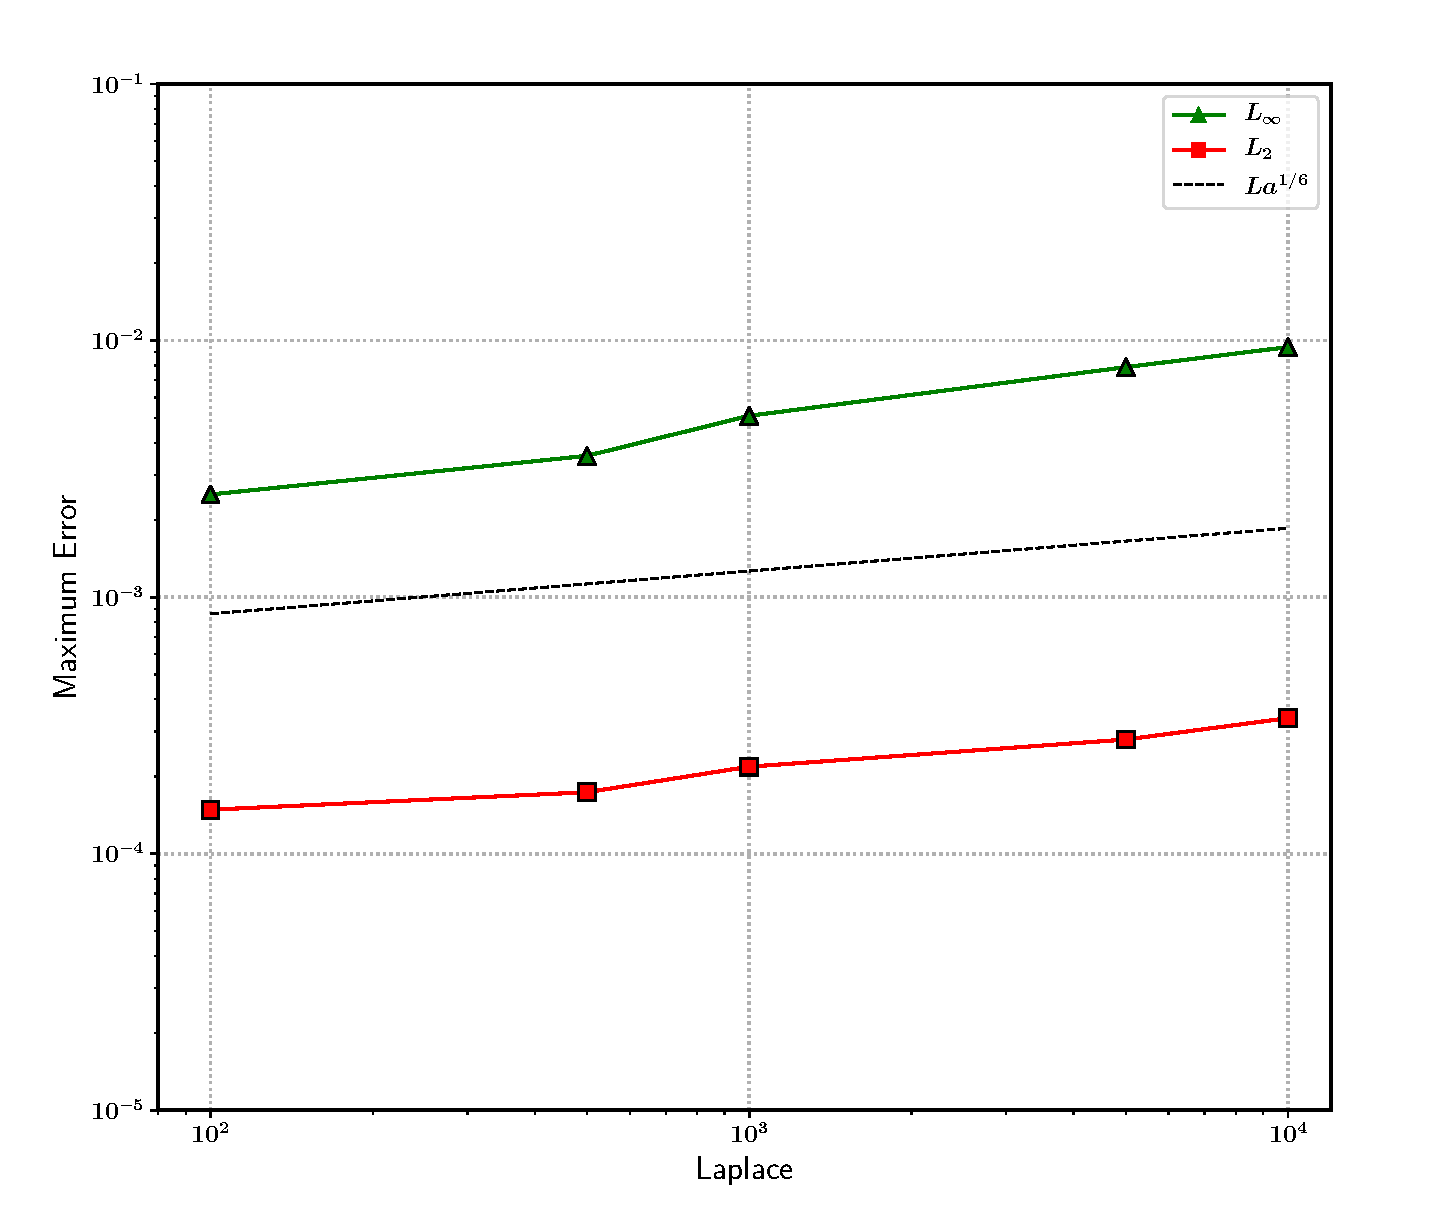
\includegraphics[width = 1.0\textwidth]{plots/droplet_advect/laplaces.pdf}
\caption{ Scaling of the maximum error norm as a function of Laplace ($We = 0.4$, $\rho_l / \rho_g = 1000$). }
    \label{lap}
\end{figure}



%------------------------------------------ CAPILLARY WAVE ---------------------------------------------

\section{Capillary Wave}
One of the fundamental features of immiscible multiphase flows involving interfaces are the presense and propagation of capillary waves. Therefore, a robust and accurate numerical method should not only be able to adequately resolve, but also accurately emulate the spatio-temporal evolution of such surface tension induced oscillations. A brief outline on the state-of-the-art numerical implementations of capillary waves (and surface tension models in general) existing in current literature is provided by Popinet in the comprehensive review \sidecite{popinet2018numerical}.

\subsection*{Setup}

\begin{figure}[h!]
    \centering
    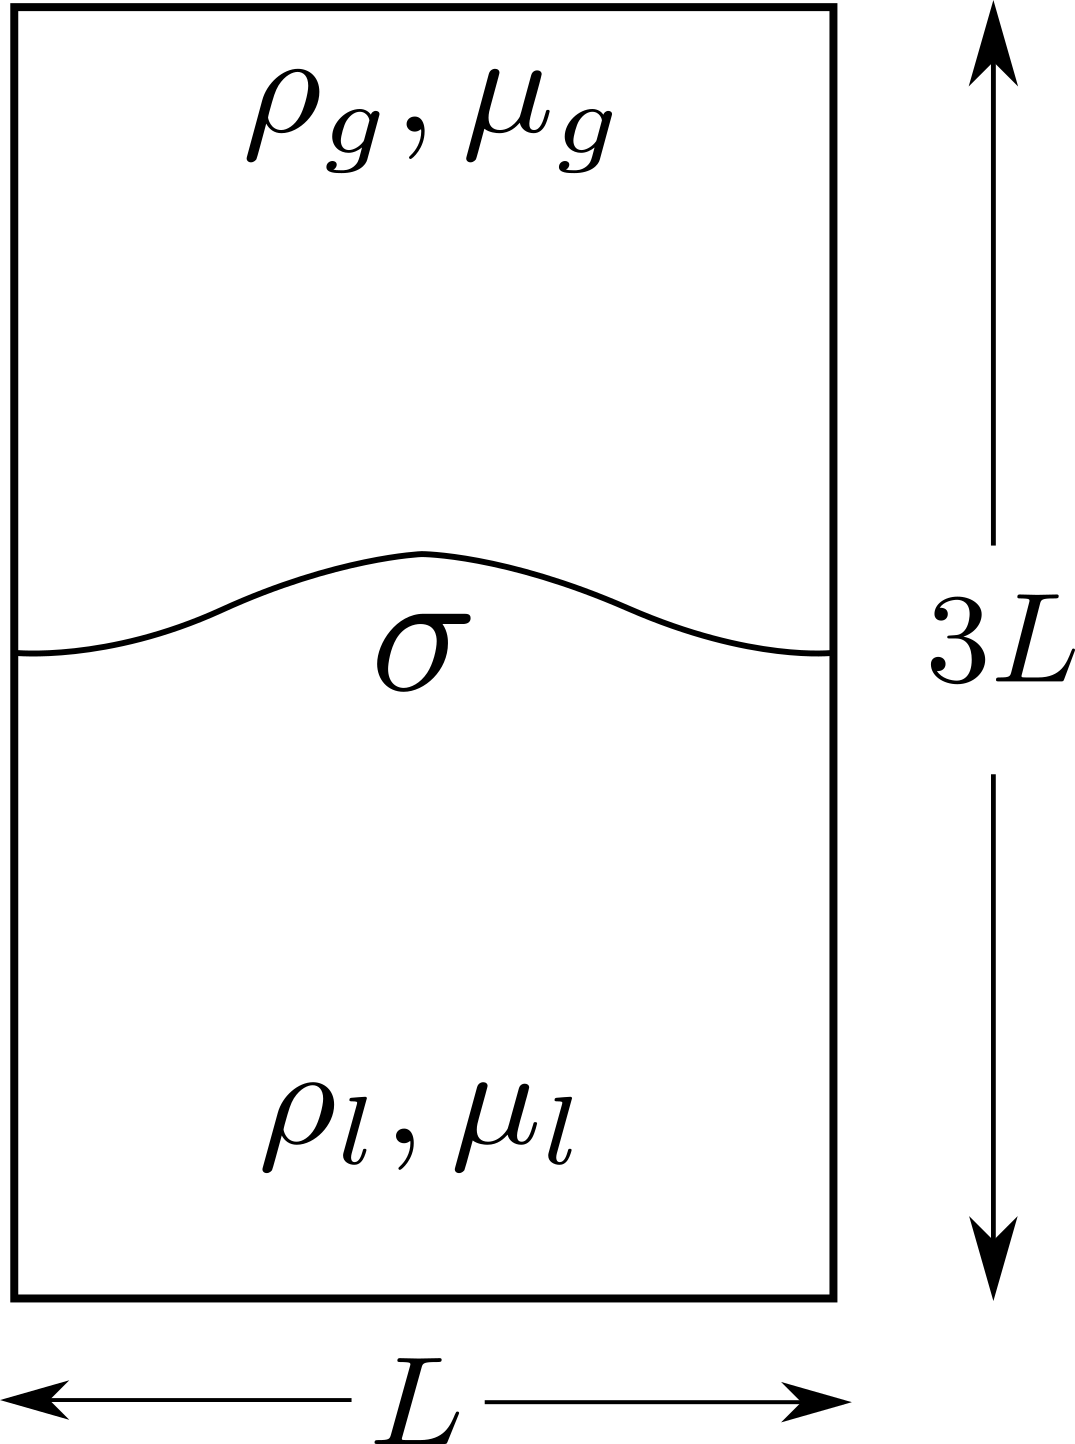
\includegraphics[width = 1.0\textwidth]{plots/capwave/capwave_conf.png}
	\caption{Schematic of the initially perturbed planar interface separating two immiscible fluids of different densities and viscosities. A spatial resolution of $32 \times 96$ is used for spatial discretization (compared to $64 \times 192$ in Popinet \cite{popinet2009accurate}), with the width of the box corresponding to the size of the perturbed wavelength.}
    \label{capwave_conf}
\end{figure}

In the present study, we evaluate the accuracy of our class of methods by comparing with an analytical solution of damped capillary oscillations. Generally, analytical solutions exist only for cases corresponding to extremely small initial perturbations, that too either in the inviscid limit (Lamb \sidecite{lamb1993hydrodynamics}) or the asymptotic limit of vanishing viscosity (Prosperetti \sidecite{prosperetti1980free,prosperetti1981motion}). For our purposes, we use the configuration of the viscosity-damped capillary oscillations of a planar interface, as was first implemented and popularized by Popinet \& Zaleski \cite{popinet1999front}.  

We consider a rectangular domain of dimensions $L \times 3L$, where $L$ corresponds to the wavelength of our initial perturbation. The densities of the heavier and lighter phases are $\rho_l$ and $\rho_g$ respectively, likewise for the viscosities $\mu_l$ and $\mu_g$, and $\sigma$ being the surface tension coefficient (fig. \ref{capwave_conf}). An intial perturbation amplitude of $L/100$ is used, coupled with a numerical resolution given by $L/\Delta x= 32$ ($\Delta x$ being the grid size). Symmetry conditions are applied on the top and bottom sides, with periodic conditions along the horizontal direction. We use the following adimensional parameters to characterize our problem : 

\begin{align}
	T_0 = T \omega_0 \quad , \quad La = \frac{\rho_l \sigma L}{\mu_l^2}  
\end{align}

where $La$ is the Laplace number based on the heavier fluid, and $\omega_0$ is defined using the dispersion relation used in Popinet \cite{popinet2009accurate} given as : 

\begin{align}
	\omega_0^2 =  \frac{\sigma k^3}{2 \rho_l} \quad, \qquad \text{where} \quad k = \frac{2\pi}{L}   
\end{align}

The dispersion relation is obtained via linear stability analysis at the inviscid limit \sidecite{lamb1993hydrodynamics}. In order to evaluate the influence of density-ratio on the performance of our class of methods, we use three different numerical setups keeping the same Laplace number ($La = 3000$) as follows : 

\begin{itemize}
	\item $\rho_l/\rho_g = 1$ , $\mu_l/\mu_g = 1$  (Popinet \cite{popinet2009accurate}) 
	\item $\rho_l/\rho_g = 10$ , $\mu_l/\mu_g = 1$   
	\item $\rho_l/\rho_g = 1000.0/1.2$ , $\mu_l/\mu_g = 1.003\cdot 10^{-3}/1.8\cdot 10^{-5}$ (Air-Water) 
\end{itemize}

The final setup corresponds to that of an air-water interface (physical properties corresponding to $20^o$ Celsuis), which is the most stringent due to the significant density and viscosity jumps. 

\subsection*{Comparison with Prosperetti Solution}

The theoretical solution to this configuration corresponds to the closed-form expressions of the planar interface shape evolution established by Prosperetti \cite{prosperetti1981motion,prosperetti1980free}, which takes into account the finite time-scales at which the vorticity (generated due to interface oscillations) diffuses into the bulk medium. These closed-form expressions are subsequently integrated using a fourth-order Runge-Kutta time integrator (details of which not described here), and used to assess the accuracy of the results obtained by our class of numerical methods. 


\begin{figure}[h!]
    \centering
    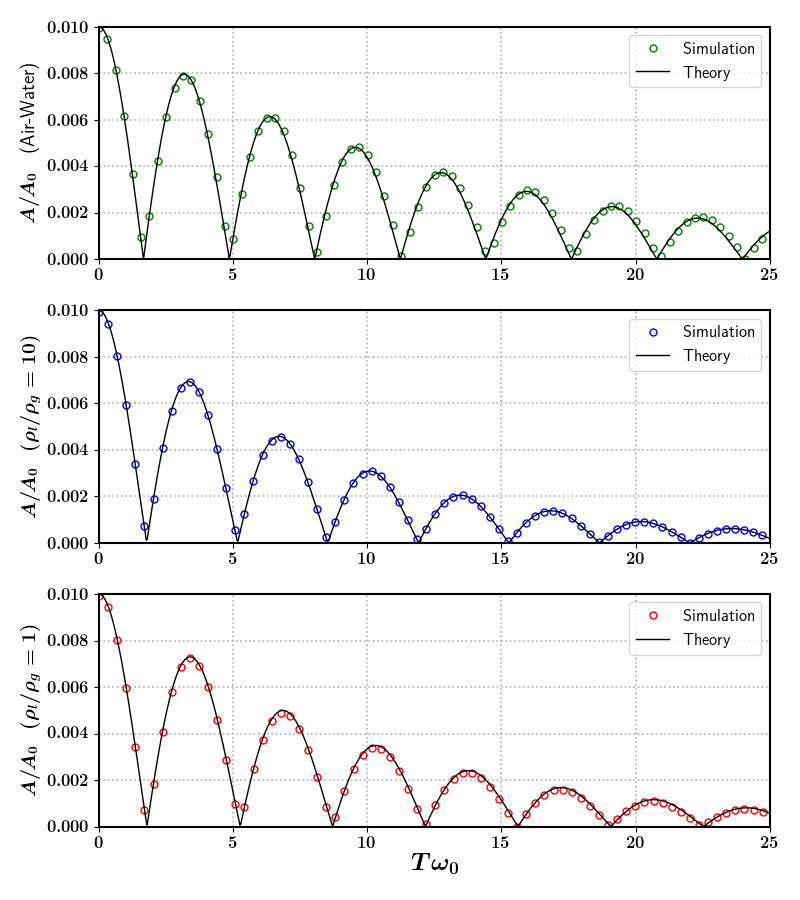
\includegraphics[width = 1.0\textwidth]{plots/capwave/compare_nonmc.png}
	\caption{\textbf{STD} Time evolution of the amplitude of the planar interface undergoing damped capillary oscillations, comparing the solution obtained by our numerical method with the closed-from Prosperetti solution. More or less good agreement with theory is observed for all the density-ratios tested. }
    \label{capwave_nonmc}
\end{figure}

As we can in figures \ref{capwave_nonmc} to \ref{capwave_sagar}, solutions from our class of numerical methods (circles) are compared to that of the theoretical (Prosperetti) solution (black curves), where the amplitude is normalized by the initial value ($A_0$) and the time rescaled by $T_0$. The first figure (\ref{capwave_nonmc}) refers to simulations carried out by the non-consistent method, the second (\ref{capwave_daniel}) corresponds to that of the consistent method, and the final one (\ref{capwave_sagar}) refers to that of the consistent and conservative method. We observe that there is hardly any appreciable qualitative difference between the results obtained via the different methods \textbf{STD}, \textbf{MSHIFT} and \textbf{MSUB}, although \textbf{MSUB} does seem to perforn marginally better when it comes to the most stringent case (air-water configuration). Surprisingly, even the non-consistent method (\textbf{STD}) does not seem to show any un-physical interfacial deformations for all the density-ratios tested, and that it is difficult to distinguish between the different methods for the lower density-ratios.  

\begin{figure}[h!]
    \centering
    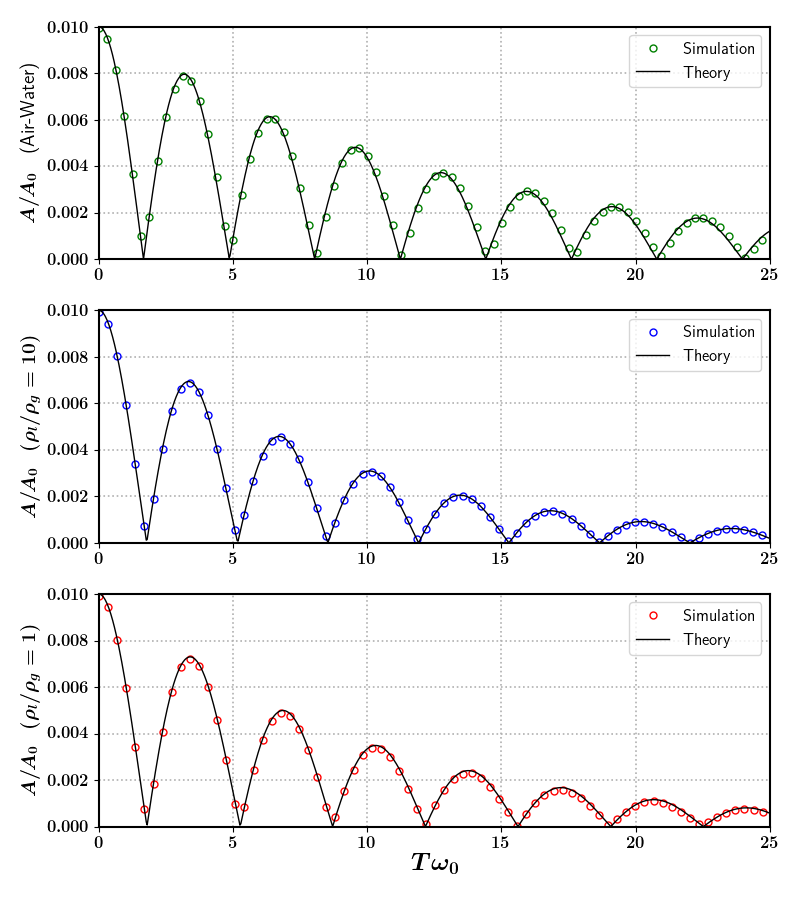
\includegraphics[width = 1.0\textwidth]{plots/capwave/compare_daniel.png}
	\caption{\textbf{MSHIFT} Time evolution of the amplitude of the planar interface undergoing damped capillary oscillations, comparing the solution obtained by our numerical method with the closed-from Prosperetti solution. Behavior is quite similar to \textbf{STD}, with good agreement with theory for all the density-ratios tested. }
    \label{capwave_daniel}
\end{figure}

\begin{figure}[h!]
    \centering
    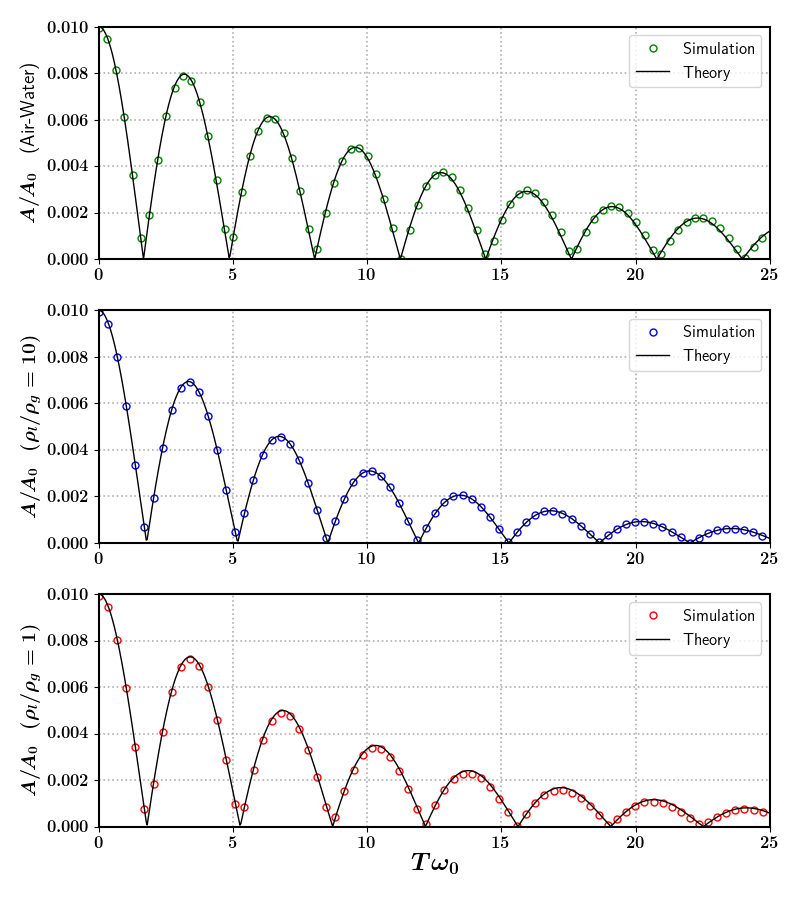
\includegraphics[width = 1.0\textwidth]{plots/capwave/compare_sagar.png}
	\caption{\textbf{MSUB} Time evolution of the amplitude of the planar interface undergoing damped capillary oscillations, comparing the solution obtained by our numerical method with the closed-from Prosperetti solution. Slightly better agreement with theory when comparing to \textbf{STD} and \textbf{MSHIFT}, for all density-ratios tested. }
    \label{capwave_sagar}
\end{figure}


\subsection*{Spatial Convergence}

The next step in our evaluation would be to quantify the accuracy of our numerical results to the Prosperetti solution using an integral (in time) error norm, the same as defined in \cite{popinet2009accurate} :       


\begin{figure}[h!]
    \centering
    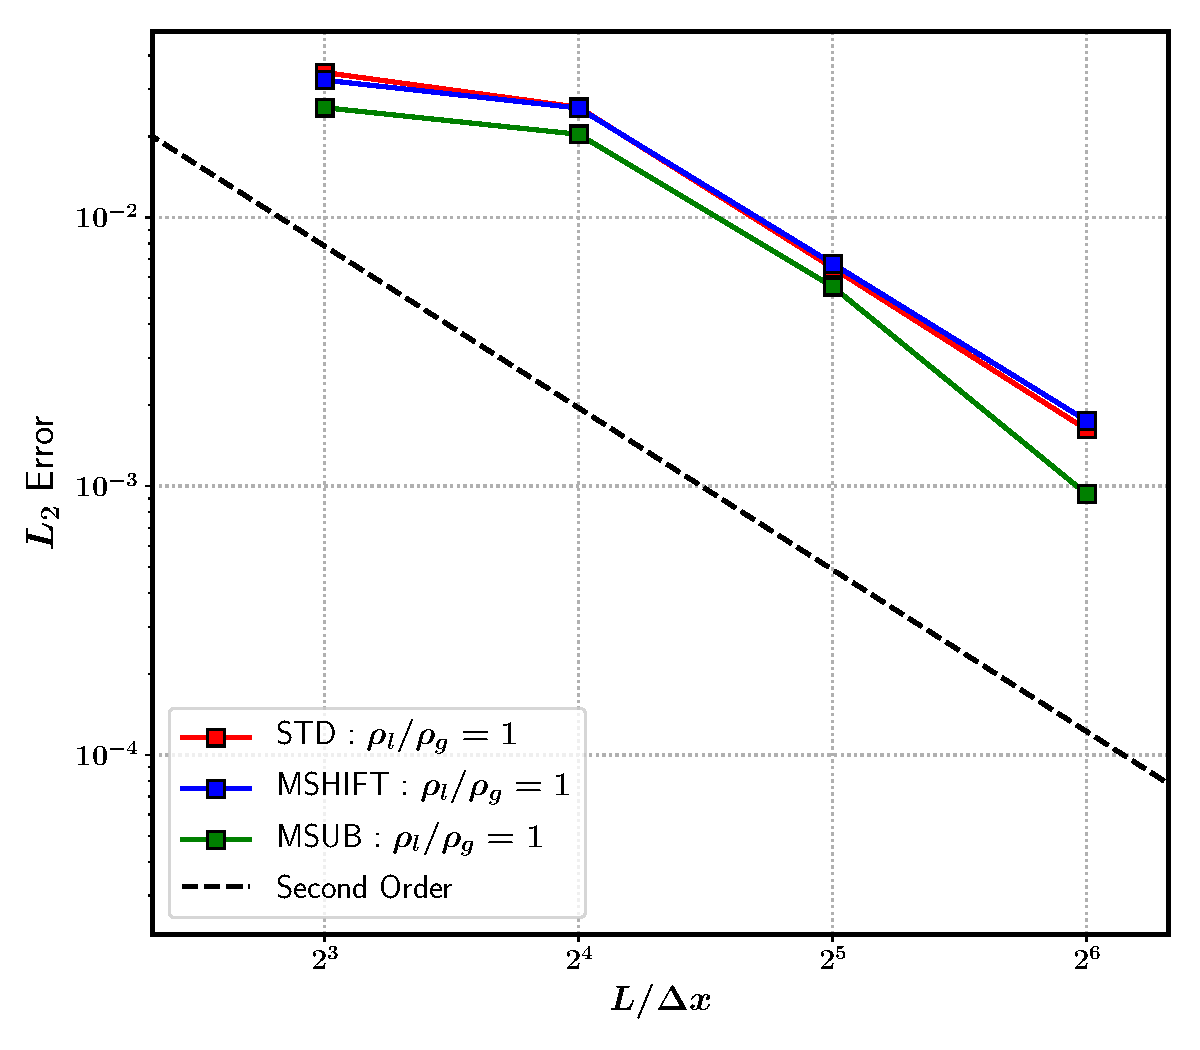
\includegraphics[width = 1.0\textwidth]{plots/capwave/conv_r1.pdf}
	\caption{Comparison of spatial convergence for the case of $\rho_l/\rho_g = 1 , La = 3000$, for our class of methods. There is no viscosity jump across the interface. All methods seem to demonstrate approximately second-order convergence. There seems to be no appreciable difference in the behavior of \textbf{STD} and \textbf{MSHIFT}, with \textbf{MSUB} displaying marginally lower errors compared to the others. }
    \label{conv_r1}
\end{figure}


\begin{figure}[h!]
    \centering
    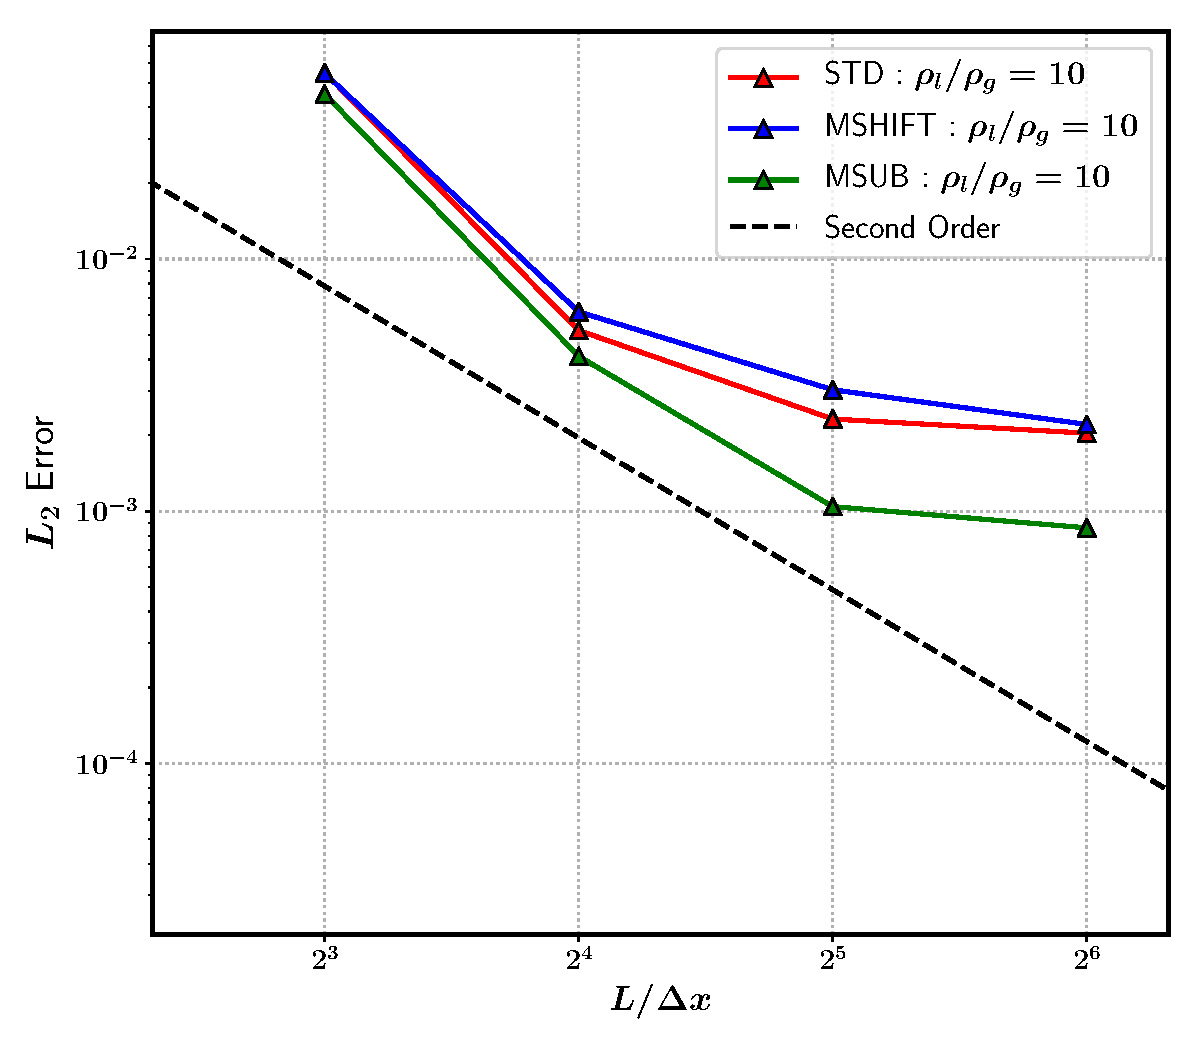
\includegraphics[width = 1.0\textwidth]{plots/capwave/conv_r10.pdf}
	\caption{Comparison of spatial convergence for the case of $\rho_l/\rho_g = 10 , La = 3000$, for our class of methods. Again, there is no viscosity jump across the interface. All methods seem to demonstrate approximately second-order convergence upto $ L/ \Delta x = 32 $, beyond which there is a slight saturation in the rate of convergence. Qualitatively, \textbf{STD} and \textbf{MSHIFT} demonstrate similar behavior, with \textbf{MSUB} delivering the lowest errors. In case of \textbf{MSUB}, the errors are lower by a factor of $2$ compared to \textbf{STD} and \textbf{MSHIFT} for resolutions above $L / \Delta x = 16$. }
    \label{conv_r10}
\end{figure}


\begin{figure}[h!]
    \centering
    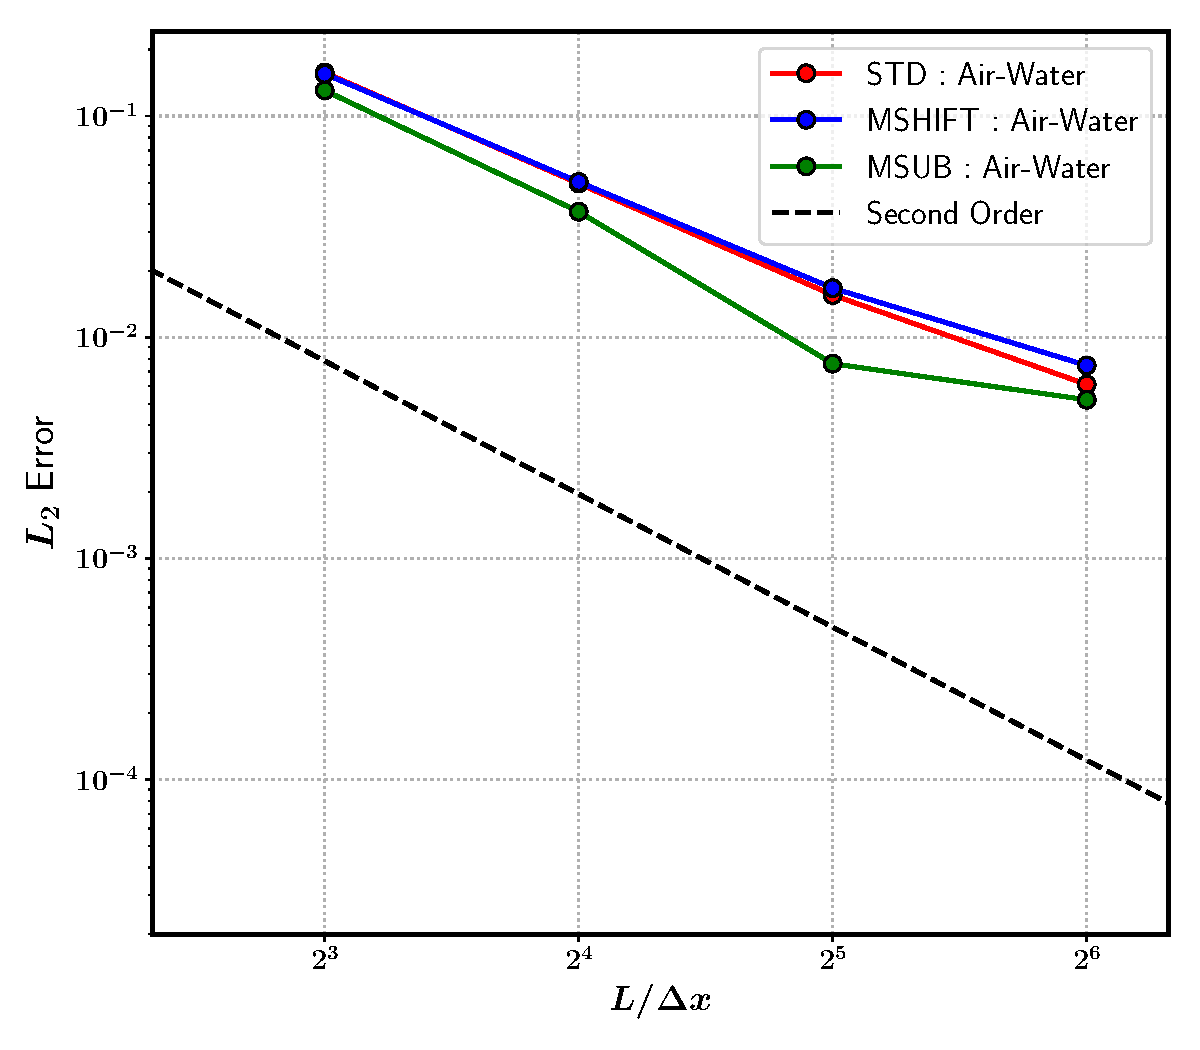
\includegraphics[width = 1.0\textwidth]{plots/capwave/conv_aw.pdf}
	\caption{Comparison of spatial convergence for the Air-Water case corresponding to $\rho_l/\rho_g = 1000.0/1.2 , \mu_l/\mu_g = 1.003\cdot 10^{-3}/1.8\cdot 10^{-5} , La = 3000 $, for our class of methods. All methods seem to demonstrate approximately second-order convergence. No appreciable difference is observed between \textbf{STD} and \textbf{MSHIFT}, with \textbf{MSUB} delivering slightly lower errors although there is some saturation in the convergence rate at higher resolutions. }
    \label{conv_aw}
\end{figure}

\begin{align}
	L_2 = \frac{1}{L} \sqrt{\frac{\omega_0}{25} \int_{t=0}^{T} \left(h - h_{exact}\right)^2}
\end{align}

where $h$ is the maximum inteface height obtained using our numerical simulations, and $h_{exact}$ being the maximum height obtained via time integration of the Prosperetti solution. In figures \ref{conv_r1} to \ref{conv_aw} we demonstrate the rate of spatial convergence of the $L_2$ error norms for different density-ratios, simultaneously comparing the behavior of the different methods \textbf{STD}, \textbf{MSHIFT} and \textbf{MSUB} at each density-ratio. In all the results presented, we maintain $La = 3000$ for all density-ratios, spatial resolutions and methods tested.  

In figure \ref{conv_r1} we observe roughly second-order spatial convergence when it comes to equal densities across the interface, with \textbf{STD} and \textbf{MSHIFT} displaying nearly identical behavior, whereas \textbf{MSUB} does marginally better with lower errors for all resolutions. When it comes to $\rho_l / \rho_g = 10$ in figure \ref{conv_r10}, we observe a saturation in the initial second-order convergence rate irrespective of whichever method is used, however \textbf{MSUB} performs much better in terms of error when compared \textbf{STD} and \textbf{MSHIFT}. Finally, figure \ref{conv_aw} demonstrates the roughly second-order convergence of all three methods when it comes to the air-water configuration, again, with \textbf{MSUB} performing merginally better with lower errors. Not surprisingly, the largest errors arise for the air-water configuration errors across all methods. 


